Nel corso dell'elaborato si è fatto riferimento alla versione Cubic del TCP, come metro di giudizio per le prestazioni di BBR. In quest'appendice si richiamano alcuni aspetti del Cubic, utili a chiarire alcuni dei suoi principali comportamenti. \bigskip

Tale appendice non è da considerarsi come fonte principale per lo studio di Cubic. Per una trattazione approfondita si suggerisce la lettura di \cite{ietf:draft-ietf-tcpm-cubic-05}, e \cite{Ha:2008:CNT:1400097.1400105}.

\section{Motivazione}

La motivazione principale che ha portato alla nascita di Cubic, riguarda un problema presentato dalle versioni Reno, e New Reno, su path di comunicazione caratterizzati da livelli elevati di RTT. \bigskip

Tali algoritmi, durante la fase di \textit{Congestion Avoidance}, eseguono un incremento della \texttt{cwnd} di una SMSS per ogni RTT. Questo causa un lento incremento della finestra, per path caratterizzati da alti valori del \textit{BDP}. \bigskip

Per esempio, con un bottleneck rate di 10Gbps e 100ms di RTT, il \textit{BDP} è di 100.000 pacchetti, se questi hanno una dimensione di 1250 Byte. Questo significa che per incrementare la \texttt{cwnd}, da \textit{BDP/2} (il punto di partenza è lo \textit{Slow start}, non il \textit{Congestion Avoidance}) fino a \textit{BDP}, è necessario un tempo pari a: 50.000*RTT = 5.000 s (1.4 ore). \bigskip

Tutto ciò non porta altro che ad una forte sottovalutazione delle capacità reali del path di rete. \bigskip

Sarebbe dunque utile, essere più aggressivi nella fase d'incremento quando si è lontani dal punto di saturazione, e meno nelle sue vicinanze. \bigskip

Il Bic-TCP fu una, tra le tanti versioni, a riuscire in tale intento.

\section{Bic-TCP}

Il Bic-TCP è un algoritmo di controllo di congestione ottimizzato per i path con alti valori del \textit{BDP}. \bigskip

Per raggiungere tale risultato, durante la fase di \textit{Congestion Avoidance}, viene utilizzato un algoritmo di binary search. \bigskip

Per utilizzarlo è innanzitutto necessario nel corso del tempo, documentare i limiti della finestra di congestione:

\begin{itemize}

\item \texttt{W\_max}: ultimo valore della \texttt{cwnd} in cui si è generato un evento di packet loss, registrato prima d'entrare in \textit{Fast Recovery}.
\item \texttt{W\_min}: ultimo valore della \texttt{cwnd} in cui per un intero RTT, non si è verificato un evento di packet loss.

\end{itemize}

A questo punto in \textit{Congestion Avoidance}, ad ogni ack ricevuto:

\begin{itemize}

\item Se \texttt{cwnd} < \texttt{W\_max}, viene realizzata una binary search:

\begin{enumerate}

\item viene determinato il mid-point tra \texttt{W\_min} (pari al valore corrente di \texttt{cwnd}) e \texttt{W\_max}.

\item se non è possibile in un RTT incrementare la \texttt{cwnd} fino al mid-point, viene eseguito un incremento addittivo di un fattore costante $S_{max}$ (parametro di configurazione). In caso contrario l'incremento è dato dalla distanza rispetto il mid-point.

\item se per un RTT non si presentano eventi di loss, viene aggiornato il valore di \texttt{W\_min}, con l'attuale valore della \texttt{cwnd}. In caso contrario si riprenderà dal passo 1, all'uscita dalla fase di \textit{Fast Recovery}.

\item Finchè l'incremento non scende al di sotto  $S_{min}$ (parametro di configurazione, che segnala se si è o meno nelle vicinanze del punto di saturazione), si riparte dal passo 1.

\end{enumerate}

Nel suo insieme il binary search, dà vita ad un incremento pressochè logaritmico, molto rapido e stabile in prossimità del punto di saturazione.

\item Se \texttt{cwnd} >= \texttt{W\_max}, significa che il limite della finestra congestione ha subito una variazione. Per cui si procede con una fase d'incremento duale alla precedente, prima esponenziale e poi lineare
(Max probing).

\end{itemize}

Mettendo insieme il tutto, otteniamo l'andamento della funzione di crescita del Bic (growth function):

\begin{figure} [H]

\center
\caption{Bic growth function}
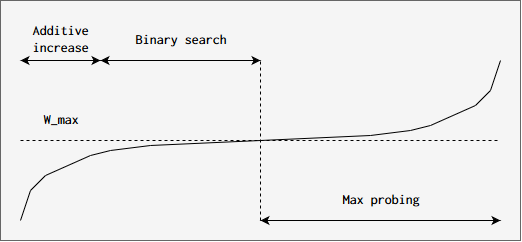
\includegraphics[scale=0.8]{chapters/A_cubic/img/growth_function.png}

\end{figure}

La forza del Bic, può essere desunta dal plateau che si forma nell'intorno di \texttt{W\_max}. Quest'ultimo permette di operare con valori alti della \texttt{cwnd} (prossimi al limite), per un tempo superiore agli approcci tradizionali. \bigskip

Se dunque è comprensibile, che questo modo di modulare la finestra di congestione, aiuta quando il \textit{BDP} in gioco è elevato, è altrettanto comprensibile che un tale approccio sia sicuramente poco fair nei confronti di Reno per BDP bassi. \bigskip 

Non solo, è possibile che in alcune zone di funzionamento la Bic function produca un avanzamento della finestra di congestione più lento rispetto quello lineare. Ciò può accadere quando si è lontani dal punto di saturazione. \bigskip

Tutto ciò congiuntamente al fatto che la realizzazione di un binary search algorithm, non è cosa semplice, ha portato allo sviluppo di Cubic.

\section{Cubic}

Cubic è un'evoluzione del Bic-TCP, di cui uno degli scopi è proprio quello di migliorare gli aspetti negativi di quest'ultimo. \bigskip

Non è infatti basato sull'utilizzo del binary search algorithm, ma sulla Cubic function:

\begin{figure} [H]

\center
\caption{Cubic growth function}
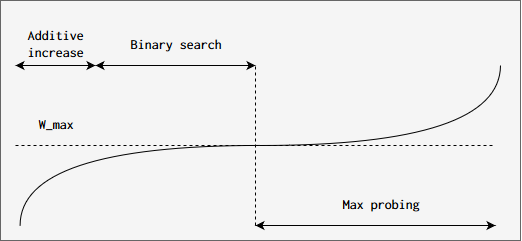
\includegraphics[scale=0.8]{chapters/A_cubic/img/cubic_growth_function.png}

\end{figure}

\[
W(t) = C*(t-K)^{3} + W_{max}
\]

Di cui:

\begin{itemize}

\item C è un parametro che determina l'aggressività dell'algoritmo, sia in fase di incremento verso il punto di saturazione, sia in fase di probing. 

\item t rappresenta il tempo trascorso dall'ultima entrata in \textit{Fast Recovery}, in cui viene fissato il valore per \texttt{W\_max}.

\item K rappresenta il tempo necessario per portare la finestra di congestione da \texttt{W} a \texttt{W\_max}.

\end{itemize}

Sono piccole le differenze rispetto la Bic function, in quanto è sicuramente importante mantenere il buon comportamento di Bic sulle reti caratterizzate da un elevato \textit{BDP}. \bigskip

Vi è tuttavia un'altra differenza, attraverso la quale il Cubic riesce a comportarsi meglio, e ad essere più fair verso i flussi Reno, in condizioni di basso RTT, ossia la \textit{Tcp Mode}.
Infatti nel corso della fase di \textit{Congestion Avoidance}, Cubic incrementa ad ogni RTT la \texttt{cwnd} sulla base della cubic function, solo se la \texttt{cwnd} si trova al di sopra del valore che si sarebbe ottenuto con l'approccio standard (s'intende Reno,new Reno). \bigskip

In caso contrario si è evidentemente in una condizione in cui l'incremento lineare per ogni RTT, funziona meglio. Per cui il Cubic entra in \textit{Tcp Mode}, ossia opera come l'approccio standard.